\Variant{30.12.2025}
\QQ{1}{$\underbrace{222\ldots222}_{50\text{ ta}}\cdot 11$ ni hisoblang.
\Opts{$2\underbrace{44\ldots44}_{45\text{ ta }4}2$}{$\underbrace{44\ldots44}_{50\text{ ta }4}2$}{$2\underbrace{44\ldots44}_{49\text{ ta }4}2$}{$2\underbrace{44\ldots44}_{48\text{ ta }4}2$}}
\QQ{2}{Hisoblang:
\[\frac{4-\frac{1}{\frac13+\frac14}}{4+\frac{1}{\frac13-\frac14}}\]
\Opts{$\dfrac14$}{$\dfrac17$}{$\dfrac1{12}$}{$\dfrac13$}}
\QQ{3}{Fermer bozorga qovun va tarvuzni $5$ ta maşina bilan olib borayotgan bölsa va bitta maşinada faqat tarvuz yoki faqat qovun bölsa, birinçi maşinada $300$, ikkinçisida $315$, uçinçisida $330$, törtinçisida $345$, beşinçisida $390$ ta mahsulot bor. Bozorkom bitta maşinani sotib bölmagunça qolganlarini sotişga ruxsat bermasdi. Bitta maşina sotib bölingandan söng qovunlar soni tarvuzlar sonidan $3$ marta köp ekanligi aniqlandi. Qovunlarning soni neçta?
\Opts{$990$}{$1035$}{$1005$}{$1050$}}
\QQ{4}{Örik tarkibida $92\%$ suv bor. Örik quritilganda qoqining tarkibida $16\%$ suv böladi. $42$ kg örik quritilganda neça kg qoqi olinadi?
\Opts{$6$}{$3$}{$4$}{$9$}}
\QQ{5}{Ifoda ratsional böladigan $n$ ning eng kiçik natural qiymatini toping:
\[\left(\frac{2^{\frac14}\cdot4^{\frac16}\cdot3^{\frac14}}{8^{\frac23}\cdot3^{\frac16}\cdot9^{\frac14}}\right)^{n}\]
\Opts{$12$}{$6$}{$18$}{$8$}}
\QQ{6}{Hisoblang:
\[\sqrt[3]{\sqrt5+2}-\sqrt[3]{\sqrt5-2}\]
\Opts{$1$}{$\sqrt5$}{$2\sqrt5$}{$-1$}}
\QQ{7}{Hisoblang:
\[\left(52+6\sqrt{43}\right)^{\frac32}-\left(52-6\sqrt{43}\right)^{\frac32}\]
\Opts{$614$}{$244$}{$484$}{$828$}}
\QQ{8}{Agar $a>b>0>c$ bölsa, $\dfrac{|ab-c|}{ab-c}+\dfrac{|ac-b|}{ac-b}+\dfrac{|bc-a|}{bc-a}$ ni soddalaştiring.
\Opts{$2a$}{$1$}{$0$}{$-1$}}
\QQ{9}{Ösuvçi arifmetik progressiyada $S_8+S_7=26$ va $S_8\cdot S_7=144$ bölsa, $S_{15}$ ni toping.
\Opts{$150$}{$120$}{$135$}{$180$}}
\QQ{10}{$x$, $y$, $z$ sonlari kamayuvçi geometrik progressiyaning ketma-ket hadlari. $x$, $2y$, $3z$ sonlari arifmetik progressiyaning ketma-ket hadlari bölsa, geometrik progressiyaning maxrajini toping.
\Opts{$\dfrac23$}{$\dfrac12$}{$1$}{$\dfrac13$}}
\QQ{11}{Ifodani soddalaştiring:
\[\frac{(x-2)^4+(x-1)^2-1}{(x-2)(x-3)+2}\]
\Opts{$x^2-5x+8$}{$x^2+3x+2$}{$x^2-2x+3$}{$x^2-3x+2$}}
\QQ{12}{Tenglama neçta butun yeçimga ega?
\[\frac{x^3}{|x|}+10x-\frac{11x}{|x|}=0\]
\Opts{$2$ ta}{$3$ ta}{çeksiz köp yeçim}{$4$ ta}}
\QQ{13}{$f(x)=2x^2+(a-10)x+6$ funksiya nollari $x_1$ va $12x_1$ bölsa, şunday $a$ larning yiğindisini toping.
\Opts{$20$}{$23$}{$-3$}{$18$}}
\QQ{14}{Tenglama neçta haqiqiy ildizga ega?
\[8-2^x\cdot x+2^{3-x}=x\]
\Opts{$2$}{$1$}{$0$}{$3$}}
\QQ{15}{Hisoblang:
\[\cos\frac{2\pi}{7}+\cos\frac{4\pi}{7}+\cos\frac{6\pi}{7}\]
\Opts{$\dfrac12$}{$-\dfrac12$}{$\dfrac18$}{$-\dfrac18$}}
\QQ{16}{Hisoblang:
\[\frac37\left(\log_2 32+27^{\log_3 4}\right)^{\log_{69}14}+4^{\log_{\frac14}\frac1{10}}+\log_3\frac{81}{\sqrt7-\sqrt5}-\log_{\frac19}\left(12-2\sqrt{35}\right)\]
\Opts{$20$}{$24$}{$14$}{$10$}}
\QQ{17}{$x^3-(x+1)^2=2001$ tenglama neçta haqiqiy yeçimga ega?
\Opts{$0$}{$1$}{$2$}{$3$}}
\QQ{18}{Tengsizlikni qanoatlantiruvçi butun sonlar neçta?
\[\bigl||x+1|-3\bigr|\le 6\]
\Opts{$18$}{$20$}{$19$}{$21$}}
\QQ{19}{Tengsizlikni neçta butun son qanoatlantiradi?
\[\sqrt{x-8\sqrt{8+x}+24}-\frac{16+x}{2\sqrt{8+x}-10}<0\]
\Opts{$10$}{$11$}{$230$}{$231$}}
\QQ{20}{Soddalaştiring:
\[\cos2\alpha+\sin2\alpha\cdot\tg\alpha\]
\Opts{$0$}{$1$}{$\sin^2\alpha$}{$\cos^2\alpha$}}
\QQ{21}{Agar $f(x+1)=x^2+2x+2$ bölsa, $f(-3)+f(1)$ ning qiymatini toping.
\Opts{$10$}{$12$}{$2$}{$14$}}
\QQ{22}{$y=\sqrt{\dfrac72x^2-7}$ funksiya grafigiga ötkazilgan urinma $y=ax+b$ bölsin. Agar $y=-\dfrac12x+3$ töğri çiziq grafigi $y=ax+b$ funksiya bilan özaro perpendikulyar bölsa, $a+b$ ning qiymatini toping.
\Opts{$1$}{$7$}{$-1$}{$3$}}
\QQ{23}{Aniq integralni hisoblang:
\[\int_0^{\frac{\pi}{12}}\left(\sin^4 3x+\cos^4 3x\right)dx\]
\Opts{$\dfrac{\pi}8$}{$\dfrac{\pi}{16}$}{$\dfrac{\pi}4$}{$\dfrac{\pi}2$}}
\QQ{24}{$ABCD$ parallelogrammning $B$ ötmas burçagi $120^\circ$ ga teng. $BC$ tomondan $E$ nuqta olingan. Agar $\bigl|\overrightarrow{AE}+\overrightarrow{BD}+\overrightarrow{EC}\bigr|=16$ va $\bigl|\overrightarrow{AE}-\overrightarrow{BD}+\overrightarrow{EC}\bigr|=10$ bölsa, $AED$ uçburçakning yuzini toping.
\qfig{\begin{tikzpicture}[scale=0.42,font=\small]
\coordinate (A) at (0,0); \coordinate (D) at (8,0); \coordinate (B) at (2.5,4.33); \coordinate (C) at (10.5,4.33); \coordinate (E) at (8.2,4.33);
\fill[qfill] (A)--(E)--(D)--cycle;
\draw (A)--(B)--(C)--(D)--cycle; \draw (A)--(E)--(D); \draw (B)--(D);
\node[below left] at (A) {$A$}; \node[above left] at (B) {$B$}; \node[above right] at (C) {$C$};
\node[below right] at (D) {$D$}; \node[above] at (E) {$E$};
\end{tikzpicture}}
\Opts{$10\sqrt3$}{$20\sqrt3$}{$8\sqrt3$}{$18\sqrt3$}}
\QQ{25}{$ABC$ töğri burçakli uçburçakning gipotenuzasiga tuşgan $CM$ mediana uzunligi katetlaridan birining uzunligiga teng. Agar $CM=2$ bölsa, $ABC$ uçburçak yuzini toping.
\Opts{$3\sqrt3$}{$6$}{$2\sqrt3$}{$3$}}
\QQ{26}{$ABC$ töğri burçakli uçburçakka töğri burçagi umumiy bölgan $ADEF$ kvadrat içki çizildi. Agar $BE=10$ va $EC=15$ bölsa, $ADEF$ kvadratning yuzini toping.
\qfig{\begin{tikzpicture}[scale=0.62,font=\small]
\coordinate (A) at (0,0); \coordinate (B) at (0,3.2); \coordinate (C) at (4.8,0);
\coordinate (D) at (0,1.92); \coordinate (E) at (1.92,1.92); \coordinate (F) at (1.92,0);
\fill[qfill] (A)--(D)--(E)--(F)--cycle;
\draw (A)--(B)--(C)--cycle; \draw (D)--(E)--(F); \draw (0,0.22)--(0.22,0.22)--(0.22,0);
\node[above left] at (B) {$B$}; \node[below left] at (A) {$A$}; \node[below right] at (C) {$C$};
\node[left] at (D) {$D$}; \node[above right] at (E) {$E$}; \node[below] at (F) {$F$};
\node[above right] at (0.96,2.56) {$10$}; \node[above right] at (3.36,0.96) {$15$};
\end{tikzpicture}}
\Opts{$69\dfrac5{13}$}{$69\dfrac3{13}$}{$67\dfrac4{13}$}{$68\dfrac2{13}$}}
\QQ{27}{$ABCD$ — parallelogramm tasvirlangan. Agar $\angle BAD=60^\circ$, $\left(\dfrac{|AC|}{|BD|}\right)^2=\dfrac{19}{7}$ va $AD>AB$ bölsa, $AD:AB$ ning qiymatini toping.
\Opts{$4:3$}{$3:1$}{$3:2$}{$2:1$}}
\QQ{28}{Aylanadagi $A$ nuqtadan uzunliklari $\sqrt{2+\sqrt3}$ va $\sqrt3$ ga teng bölgan $AB$ va $AC$ vatarlar ötkazilgan. Agar $AB$ va $AC$ vatarlar orasidagi burçak $45^\circ$ ga teng bölsa, aylana markazidan $AC$ vatargaça bölgan masofani toping.
\qfig{\begin{tikzpicture}[scale=1.5,font=\small]
\coordinate (O) at (0,0); \coordinate (A) at (165:1); \coordinate (B) at (15:1); \coordinate (C) at (-75:1);
\coordinate (H) at ($(A)!0.5!(C)$);
\draw (O) circle (1); \draw (A)--(B); \draw (A)--(C); \draw (O)--(H);
\draw ($(H)!0.09!(O)$) -- ($($(H)!0.09!(O)$)!0.09/0.5!-90:(H)$);
\fill (O) circle (0.9pt);
\node[left] at (A) {$A$}; \node[right] at (B) {$B$}; \node[below] at (C) {$C$}; \node[above right] at (O) {$O$};
\node[above] at ($(A)!0.5!(B)$) {$\sqrt{2+\sqrt3}$}; \node[below left] at ($(A)!0.55!(C)$) {$\sqrt3$};
\node at ($(A)+(-30:0.3)$) {\scriptsize$45^\circ$};
\end{tikzpicture}}
\Opts{$1$}{$\dfrac{\sqrt3}2$}{$\dfrac12$}{$\dfrac14$}}
\QQ{29}{Muntazam ön ikki burçakning tomoni $2$ ga teng bölsa, böyalgan soha yuzini toping.
\qfig{\begin{tikzpicture}[scale=1.15,font=\small]
\fill[qfill] (165:1)--(15:1)--(45:1)--cycle;
\draw (15:1) \foreach \k in {1,...,11} {--({15+30*\k}:1)} --cycle;
\draw (165:1)--(15:1); \draw (165:1)--(45:1);
\node[right] at ($(15:1)!0.5!(45:1)$) {$2$};
\end{tikzpicture}}
\Opts{$3+2\sqrt3$}{$2\sqrt2+\sqrt6$}{$3+2\sqrt2$}{$4+2\sqrt2$}}
\QQ{30}{Tekislikda yotmagan nuqtadan tekislikka oğma va perpendikulyar tuşirilgan. Oğma va tekislik orasidagi burçak $\arccos0{,}28$ bölsa, oğmaning tekislikdagi proyeksiyasi $21$ bölsa, perpendikulyar uzunligini toping.
\Opts{$75$}{$48$}{$64$}{$72$}}
\QQ{31}{Agar $A=\{(x,y)\mid x^2+y^2=9;\ x,y\in\mathbb R\}$ va $B=\{(x,y)\mid x+y=3;\ x,y\in\mathbb R\}$ bölsa, $A\cap B$ ni toping.
\Opts{$\{(-3;0);\ (0;-3)\}$}{$\{(3;0);\ (0;3)\}$}{$\{(-3;3);\ (3;-3)\}$}{$\{(-3;0);\ (0;2)\}$}}
\QQ{32}{Binomial yoyilmaning koeffitsiyentlar yiğindisini toping:
\[C_{99}^1+C_{99}^3+C_{99}^5+\ldots+C_{99}^{99}\]
\Opts{$2^{98}$}{$2^{98}-1$}{$2^{99}-1$}{$2^{99}$}}
\QQ{33}{\Moslash{$SABCD$ muntazam törtburçakli piramidaning yon yoqlari asos tekisligi bilan $30^\circ$ li burçak taşkil etadi. Bu piramidaga asosi piramida asosida va yon yoqlariga urinuvçi yarim şar içki çizilgan. Piramida asosi tomonidan yarim şar diametri ayirmasi $1$ ga teng. ($\pi\approx3$ deb hisoblang.)
\par\centering\begin{tikzpicture}[scale=1.05,font=\small]
\coordinate (A) at (-1.6,0.45); \coordinate (B) at (1.6,0.45); \coordinate (C) at (-1,-0.55); \coordinate (D) at (2.2,-0.55);
\coordinate (O) at (0.3,-0.05); \coordinate (S) at (0.3,1.9);
\fill[qfill] (O) ++(-0.62,0) arc (180:0:0.62 and 0.6) arc (0:-180:0.62 and 0.2);
\draw[dashed] (O) ellipse (0.62 and 0.2); \draw[dashed] (O) ++(-0.62,0) arc (180:0:0.62 and 0.6);
\draw (A)--(C)--(D); \draw (S)--(A); \draw (S)--(C); \draw (S)--(D);
\draw[dashed] (A)--(B)--(D); \draw[dashed] (S)--(B);
\node[left] at (A) {$A$}; \node[right] at (B) {$B$}; \node[below] at (C) {$C$}; \node[below right] at (D) {$D$}; \node[above] at (S) {$S$};
\end{tikzpicture}}{A) $\dfrac12$\par B) $1$\par C) $\dfrac{\sqrt3}2$\par D) $\dfrac{\sqrt2}2$\par E) $\dfrac{4\sqrt3}9$\par F) $\dfrac{\sqrt3}4$}{Yarim şar radiusini toping.}{Yarim şarning piramida yon yoğiga uriniş nuqtasidan piramida asosigaça bölgan masofani toping.}{Piramida hajmini toping.}}
\QQ{36}{Tenglamani yeçing:
\[x^4-12x^2+16\sqrt2x-12=0\]
\AB{Tenglama neçta haqiqiy ildizga ega?}{Tenglamaning haqiqiy ildizlari köpaytmasini toping.}}
\QQ{37}{Tenglama berilgan:
\[\sin\left(\frac{\pi}2+x\right)+\cos3x=\cos4x+1\]
\AB{Tenglamaning eng kiçik musbat ildizini toping.}{$[0;\,\pi]$ oraliqdagi ildizlari sonini toping.}}
\QQ{38}{Quyidagi $f(x)$ va $g(x)$ funksiyalar uçun $f(x)=x^2+12x+30$ va $g(x)=f(f(f(f(f(x)))))$ bölsin.
\AB{$g(x)=0$ tenglama neçta haqiqiy ildizga ega?}{$g(-5)$ ning qiymatini toping.}}
\QQ{39}{$f(x)=-x^4-2x^3+3x^2+\dfrac{14x}3+2$ funksiya ikkita lokal maksimum, bitta lokal minimum nuqtaga ega. $g(x)=kx+l$ funksiya uning ikkita nuqtasiga urinadi.
\AB{$k+l$ ning qiymatini toping.}{$f(x)$ va $g(x)$ funksiyalarning uriniş nuqtalari orasidagi masofani toping.}}
\QQ{40}{Rasmda $y=a\cos(kx)+b$ funksiya grafigi tasvirlangan.
\qfig{\begin{tikzpicture}[x=0.55cm,y=0.42cm,font=\small]
\fill[qfill,domain=2:6,samples=80,variable=\t] plot ({\t*pi/3.1416*1},{2*cos(\t*90)+2}) -- plot[domain=6:2] ({\t*pi/3.1416*1},{-2*cos(\t*90)-2}) -- cycle;
\draw[->] (-0.4,0)--(8.6,0) node[right] {$x$}; \draw[->] (0,-5.2)--(0,5.4) node[above] {$y$};
\draw[dashed] (0,4)--(8.5,4); \draw[dashed] (0,-4)--(8.5,-4);
\draw[thick,domain=0:8.3,samples=120,variable=\t] plot ({\t},{2*cos(\t*90)+2});
\draw[domain=2:6,samples=80,variable=\t] plot ({\t},{-2*cos(\t*90)-2});
\node[left] at (0,4) {$4$}; \node[left] at (0,-4) {$-4$};
\draw (2,0.15)--(2,-0.15) node[below] {$2\pi$}; \draw (6,0.15)--(6,-0.15) node[below] {$6\pi$};
\node[above] at (4.2,4) {$y=a\cos(kx)+b$};
\end{tikzpicture}}
\AB{$\dfrac{a+b}{k}$ ning qiymatini toping.}{$[2\pi;\,6\pi]$ oraliqda funksiyani $Ox$ öqi atrofida $360^\circ$ ga aylantirişdan hosil bölgan jism hajmini toping.}}
\QQ{41}{Markazlari $O_1$, $O_2$, $O_3$ va $O_4$ bölgan teng aylanalar $ABCD$ rombga rasmda körsatilgandek içki çizilgan: $O_1$ va $O_2$ aylanalar özaro va $AD$ tomonga, $O_3$ va $O_4$ aylanalar özaro va $BC$ tomonga urinadi; $O_1$ aylana $AB$ ga, $O_3$ aylana $CD$ ga, $O_2$ va $O_4$ aylanalar esa $BD$ diagonalga urinadi. Agar $BD=12$, $AD=10$ bölsa,
\qfig{\begin{tikzpicture}[scale=0.36,font=\small]
\coordinate (A) at (0,0); \coordinate (D) at (10,0); \coordinate (B) at (2.8,9.6); \coordinate (C) at (12.8,9.6);
\coordinate (O1) at (2.5,1.875); \coordinate (O2) at (6.25,1.875); \coordinate (O3) at (10.3,7.725); \coordinate (O4) at (6.55,7.725);
\fill[qfill] (O1)--(O2)--(O3)--(O4)--cycle;
\draw (A)--(B)--(C)--(D)--cycle; \draw (B)--(D); \draw (A)--(C);
\foreach \o in {O1,O2,O3,O4} {\draw (\o) circle (1.875); \fill (\o) circle (2.5pt);}
\draw (O1)--(O2)--(O3)--(O4)--cycle;
\node[below left] at (A) {$A$}; \node[above left] at (B) {$B$}; \node[above right] at (C) {$C$}; \node[below right] at (D) {$D$};
\node[below] at (O1) {$O_1$}; \node[below] at (O2) {$O_2$}; \node[right] at (O3) {$O_3$}; \node[above] at (O4) {$O_4$};
\node[left] at (1.4,4.8) {$10$}; \node[below] at (5,0) {$10$};
\end{tikzpicture}}
\AB{$O_1$ va $O_3$ aylana markazlari orasidagi masofani toping.}{$O_1O_2O_3O_4$ törtburçak yuzini toping.}}
\QQ{42}{$ABC$ muntazam uçburçak içidan $P$ nuqta olinib, uçburçak uçlari bilan tutaştirildi. $ACP$ uçburçakka markazi $O$ nuqta bölgan aylana içki çizilgan. Agar $AP=3$, $PB=5$ va $PC=\sqrt{19}$ bölsa,
\qfig{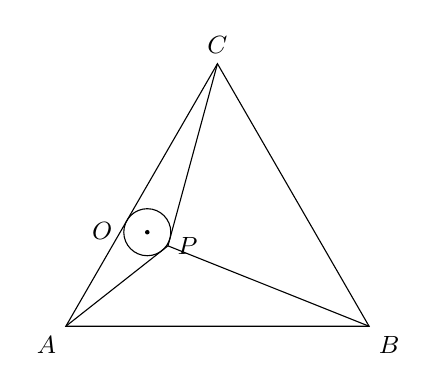
\begin{tikzpicture}[scale=0.55,font=\small]
\coordinate (A) at (0,0); \coordinate (B) at (7,0); \coordinate (C) at (3.5,6.062); \coordinate (P) at (2.357,1.856); \coordinate (O) at (1.880,2.171);
\draw (A)--(B)--(C)--cycle; \draw (A)--(P)--(B); \draw (P)--(C);
\draw (O) circle (0.543); \fill (O) circle (1.5pt);
\node[below left] at (A) {$A$}; \node[below right] at (B) {$B$}; \node[above] at (C) {$C$};
\node[right] at (P) {$P$}; \node[left] at (1.3,2.2) {$O$};
\end{tikzpicture}}
\AB{$ABC$ uçburçak perimetrini toping.}{$P$ nuqtadan aylana markazigaça bölgan masofani toping.}}
\QQ{43}{Aylanaga tomonlari soni juft bölgan muntazam köpburçak içki çizilgan. Köpburçakning bir uçidan çiqqan eng katta va eng kiçik diagonallari orasidagi burçak $60^\circ$ ga teng bölsa,
\AB{Köpburçakning diagonallari sonini toping.}{Aylana radiusi $6$ ga teng bölsa, muntazam köpburçak yuzini toping.}}
\QQ{44}{$ABCD$ muntazam tetraedrning içki sohasiga uçi $AC$ tomonning örtasida bölgan konus çizilgan. Konusning asosi tetraedrning $BC$ tomoni örtasidan ötuvçi va $BD$ va $AC$ qirralariga parallel bölgan kesimga içki çizilgan. Agar konusning yon sirti $\sqrt3\pi$ ga teng bölsa ($\pi\approx3$ deb oling),
\AB{Konus hajmini toping.}{Tetraedr hajmini toping.}}
\QQ{45}{Uyning tom qismi asosining tomonlari $8$ m va $5$ m va ular orasidagi burçak $60^\circ$ ga teng bölgan uçburçakli töğri prizmadan iborat (rasmga qarang). Tomning ikki yon yoği tunukadan iborat. Uyning pastki qismi parallelepipeddan iborat bölib, uning ikki yoği kvadrat, qolgan ikki yoği esa töğri törtburçakdan iborat.
\qfig{\begin{tikzpicture}[scale=1,font=\small]
\coordinate (E) at (0,0); \coordinate (D) at (2.4,0); \coordinate (B) at (0,2.4); \coordinate (K) at (2.4,2.4); \coordinate (A) at (1.65,3.7);
\coordinate (d) at (2.02,0.82);
\coordinate (B1) at ($(B)+(d)$); \coordinate (G) at ($(K)+(d)$); \coordinate (H) at ($(A)+(d)$); \coordinate (F) at ($(D)+(d)$); \coordinate (E1) at ($(E)+(d)$);
\draw (E)--(D)--(K)--(B)--cycle; \draw (B)--(A)--(K); \draw (A)--(H)--(G)--(K); \draw (B)--(B1)--(H); \draw (D)--(F)--(G);
\draw[dashed] (B1)--(E1)--(E); \draw[dashed] (E1)--(F);
\draw (K) ++(180:0.32) arc (180:120:0.32); \node at ($(K)+(150:0.55)$) {\scriptsize$60^\circ$};
\node[left] at (B) {$B$}; \node[above] at (A) {$A$}; \node[above] at (H) {$H$}; \node[right] at (G) {$G$};
\node[right] at (F) {$F$}; \node[below] at (D) {$D$}; \node[below left] at (E) {$E$};
\node[below] at ($(B)!0.5!(K)$) {$8$ m}; \node[right] at ($(G)!0.5!(F)$) {$8$ m}; \node[below right] at ($(D)!0.5!(F)$) {$12$ m}; \node[above right] at ($(H)!0.5!(G)$) {$5$ m};
\end{tikzpicture}}
\AB{Uyning tom qismini qoplaşga neça m$^2$ tunuka işlatilgan?}{Uyning hajmini toping (m$^3$).}}
\Javoblar{C B B C A A D D A D D A A B B A B C C B B A B A C B C C A D B A A F E}{%
\OK{36}{$2$}{$-6$}\OK{37}{$\dfrac{\pi}4$}{$4$}\OK{38}{$2$}{$-5$}\OK{39}{$\dfrac{20}3$}{$\sqrt{13}$}%
\OK{40}{$8$}{$24\pi^2$}\OK{41}{$\dfrac{39}4$}{$\dfrac{351}{16}$}\OK{42}{$21$}{$\sqrt{\dfrac{266-59\sqrt{19}}{27}}$}%
\OK{43}{$54$}{$108$}\OK{44}{$\sqrt2$}{$\dfrac{16\sqrt2}3$}\OK{45}{$144$}{$768+120\sqrt3$}}
